\documentclass[twoside]{book}

% Packages required by doxygen
\usepackage{fixltx2e}
\usepackage{calc}
\usepackage{doxygen}
\usepackage[export]{adjustbox} % also loads graphicx
\usepackage{graphicx}
\usepackage[utf8]{inputenc}
\usepackage{makeidx}
\usepackage{multicol}
\usepackage{multirow}
\PassOptionsToPackage{warn}{textcomp}
\usepackage{textcomp}
\usepackage[nointegrals]{wasysym}
\usepackage[table]{xcolor}

% Font selection
\usepackage[T1]{fontenc}
\usepackage[scaled=.90]{helvet}
\usepackage{courier}
\usepackage{amssymb}
\usepackage{sectsty}
\renewcommand{\familydefault}{\sfdefault}
\allsectionsfont{%
  \fontseries{bc}\selectfont%
  \color{darkgray}%
}
\renewcommand{\DoxyLabelFont}{%
  \fontseries{bc}\selectfont%
  \color{darkgray}%
}
\newcommand{\+}{\discretionary{\mbox{\scriptsize$\hookleftarrow$}}{}{}}

% Page & text layout
\usepackage{geometry}
\geometry{%
  a4paper,%
  top=2.5cm,%
  bottom=2.5cm,%
  left=2.5cm,%
  right=2.5cm%
}
\tolerance=750
\hfuzz=15pt
\hbadness=750
\setlength{\emergencystretch}{15pt}
\setlength{\parindent}{0cm}
\setlength{\parskip}{3ex plus 2ex minus 2ex}
\makeatletter
\renewcommand{\paragraph}{%
  \@startsection{paragraph}{4}{0ex}{-1.0ex}{1.0ex}{%
    \normalfont\normalsize\bfseries\SS@parafont%
  }%
}
\renewcommand{\subparagraph}{%
  \@startsection{subparagraph}{5}{0ex}{-1.0ex}{1.0ex}{%
    \normalfont\normalsize\bfseries\SS@subparafont%
  }%
}
\makeatother

% Headers & footers
\usepackage{fancyhdr}
\pagestyle{fancyplain}
\fancyhead[LE]{\fancyplain{}{\bfseries\thepage}}
\fancyhead[CE]{\fancyplain{}{}}
\fancyhead[RE]{\fancyplain{}{\bfseries\leftmark}}
\fancyhead[LO]{\fancyplain{}{\bfseries\rightmark}}
\fancyhead[CO]{\fancyplain{}{}}
\fancyhead[RO]{\fancyplain{}{\bfseries\thepage}}
\fancyfoot[LE]{\fancyplain{}{}}
\fancyfoot[CE]{\fancyplain{}{}}
\fancyfoot[RE]{\fancyplain{}{\bfseries\scriptsize Generated by Doxygen }}
\fancyfoot[LO]{\fancyplain{}{\bfseries\scriptsize Generated by Doxygen }}
\fancyfoot[CO]{\fancyplain{}{}}
\fancyfoot[RO]{\fancyplain{}{}}
\renewcommand{\footrulewidth}{0.4pt}
\renewcommand{\chaptermark}[1]{%
  \markboth{#1}{}%
}
\renewcommand{\sectionmark}[1]{%
  \markright{\thesection\ #1}%
}

% Indices & bibliography
\usepackage{natbib}
\usepackage[titles]{tocloft}
\setcounter{tocdepth}{3}
\setcounter{secnumdepth}{5}
\makeindex

% Hyperlinks (required, but should be loaded last)
\usepackage{ifpdf}
\ifpdf
  \usepackage[pdftex,pagebackref=true]{hyperref}
\else
  \usepackage[ps2pdf,pagebackref=true]{hyperref}
\fi
\hypersetup{%
  colorlinks=true,%
  linkcolor=blue,%
  citecolor=blue,%
  unicode%
}

% Custom commands
\newcommand{\clearemptydoublepage}{%
  \newpage{\pagestyle{empty}\cleardoublepage}%
}

\usepackage{caption}
\captionsetup{labelsep=space,justification=centering,font={bf},singlelinecheck=off,skip=4pt,position=top}

%===== C O N T E N T S =====

\begin{document}

% Titlepage & ToC
\hypersetup{pageanchor=false,
             bookmarksnumbered=true,
             pdfencoding=unicode
            }
\pagenumbering{roman}
\begin{titlepage}
\vspace*{7cm}
\begin{center}%
{\Large My Project }\\
\vspace*{1cm}
{\large Generated by Doxygen 1.8.11}\\
\end{center}
\end{titlepage}
\clearemptydoublepage
\tableofcontents
\clearemptydoublepage
\pagenumbering{arabic}
\hypersetup{pageanchor=true}

%--- Begin generated contents ---
\chapter{Class Index}
\section{Class List}
Here are the classes, structs, unions and interfaces with brief descriptions\+:\begin{DoxyCompactList}
\item\contentsline{section}{\hyperlink{classGame}{Game} \\*The main \hyperlink{classGame}{Game} class. You should make a derived class from it }{\pageref{classGame}}{}
\item\contentsline{section}{\hyperlink{classGameState}{Game\+State} \\*This class contains the state of the game. It draws it, shows the output window and saves game for further viewing }{\pageref{classGameState}}{}
\item\contentsline{section}{\hyperlink{classHexMap}{Hex\+Map} \\*Useful class for using hex maps }{\pageref{classHexMap}}{}
\item\contentsline{section}{\hyperlink{classInfo}{Info} \\*Usable class for printing real-\/time info }{\pageref{classInfo}}{}
\item\contentsline{section}{\hyperlink{classMultiStream}{Multi\+Stream} \\*Class used to combining multiple streams into one }{\pageref{classMultiStream}}{}
\end{DoxyCompactList}

\chapter{File Index}
\section{File List}
Here is a list of all documented files with brief descriptions\+:\begin{DoxyCompactList}
\item\contentsline{section}{\hyperlink{Common_8h}{Common.\+h} \\*Contains some useful functions and common\+Font }{\pageref{Common_8h}}{}
\item\contentsline{section}{{\bfseries Config.\+h} }{\pageref{Config_8h}}{}
\item\contentsline{section}{{\bfseries C\+Tcp\+Fwd.\+h} }{\pageref{CTcpFwd_8h}}{}
\item\contentsline{section}{\hyperlink{Game_8h}{Game.\+h} \\*Contains the main \hyperlink{classGame}{Game} class }{\pageref{Game_8h}}{}
\item\contentsline{section}{\hyperlink{GameState_8h}{Game\+State.\+h} \\*Contains the \hyperlink{classGameState}{Game\+State} class }{\pageref{GameState_8h}}{}
\item\contentsline{section}{\hyperlink{HexMap_8h}{Hex\+Map.\+h} \\*Contains the \hyperlink{classHexMap}{Hex\+Map} class }{\pageref{HexMap_8h}}{}
\item\contentsline{section}{\hyperlink{Info_8h}{Info.\+h} \\*Contains the \hyperlink{classInfo}{Info} class }{\pageref{Info_8h}}{}
\item\contentsline{section}{\hyperlink{Log_8h}{Log.\+h} \\*Contains the \hyperlink{classMultiStream}{Multi\+Stream} class }{\pageref{Log_8h}}{}
\item\contentsline{section}{{\bfseries Properties\+Editor.\+h} }{\pageref{PropertiesEditor_8h}}{}
\item\contentsline{section}{{\bfseries Settings.\+h} }{\pageref{Settings_8h}}{}
\item\contentsline{section}{{\bfseries Stream\+Window.\+h} }{\pageref{StreamWindow_8h}}{}
\item\contentsline{section}{\hyperlink{Wrapper_8h}{Wrapper.\+h} \\*Contains a few useful functions for communication with server }{\pageref{Wrapper_8h}}{}
\end{DoxyCompactList}

\chapter{Class Documentation}
\hypertarget{classGame}{}\section{Game Class Reference}
\label{classGame}\index{Game@{Game}}


The main \hyperlink{classGame}{Game} class. You should make a derived class from it.  




{\ttfamily \#include $<$Game.\+h$>$}



Collaboration diagram for Game\+:\nopagebreak
\begin{figure}[H]
\begin{center}
\leavevmode
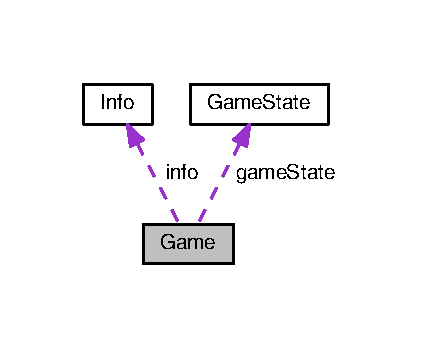
\includegraphics[width=202pt]{classGame__coll__graph}
\end{center}
\end{figure}
\subsection*{Public Member Functions}
\begin{DoxyCompactItemize}
\item 
sf\+::\+Vector2f \hyperlink{classGame_a34b9f33fe8fb922224b95e50795629c2}{get\+Mouse\+Position} ()\hypertarget{classGame_a34b9f33fe8fb922224b95e50795629c2}{}\label{classGame_a34b9f33fe8fb922224b95e50795629c2}

\begin{DoxyCompactList}\small\item\em Returns mouse cursor position after applying camera transform. \end{DoxyCompactList}\item 
void \hyperlink{classGame_a401542d59b5346cba650367e548626ce}{move\+Camera} (float cx, float cy, float zoom=1.f)
\begin{DoxyCompactList}\small\item\em Moves camera so that its centered at (cx, cy) and zoomed with specified factor. \end{DoxyCompactList}\item 
void \hyperlink{classGame_a1ab78f5ed0d5ea879157357cf2fb2afa}{run} ()
\begin{DoxyCompactList}\small\item\em This function simply runs the game until the main window is closed or an exception fired. \end{DoxyCompactList}\item 
{\footnotesize template$<$class T $>$ }\\void \hyperlink{classGame_a17b8b67b1ebc97d05b97925bfe53b61f}{add\+Drawable} (const T \&x)\hypertarget{classGame_a17b8b67b1ebc97d05b97925bfe53b61f}{}\label{classGame_a17b8b67b1ebc97d05b97925bfe53b61f}

\begin{DoxyCompactList}\small\item\em This function simply calls game\+State.\+add\+Drawable(x) \end{DoxyCompactList}\item 
void \hyperlink{classGame_a52ebfe7608394f1281efb3032d059967}{show\+Output\+Window} ()\hypertarget{classGame_a52ebfe7608394f1281efb3032d059967}{}\label{classGame_a52ebfe7608394f1281efb3032d059967}

\begin{DoxyCompactList}\small\item\em Shows window with content of mout and merr. \end{DoxyCompactList}\item 
int \hyperlink{classGame_a86c625ebc5fedb4072d007ed42d89671}{get\+Turns\+Left} ()\hypertarget{classGame_a86c625ebc5fedb4072d007ed42d89671}{}\label{classGame_a86c625ebc5fedb4072d007ed42d89671}

\begin{DoxyCompactList}\small\item\em Returns the number of turns left. \end{DoxyCompactList}\end{DoxyCompactItemize}
\subsection*{Protected Member Functions}
\begin{DoxyCompactItemize}
\item 
virtual void \hyperlink{classGame_a03387676134dd331f4a1902349926816}{draw} ()\hypertarget{classGame_a03387676134dd331f4a1902349926816}{}\label{classGame_a03387676134dd331f4a1902349926816}

\begin{DoxyCompactList}\small\item\em You can override this function for custom real-\/time drawing (which should be updated more often than once per turn) \end{DoxyCompactList}\item 
virtual void \hyperlink{classGame_a51e7f9bfbb9a2d29525b6ea009ebc345}{update} ()\hypertarget{classGame_a51e7f9bfbb9a2d29525b6ea009ebc345}{}\label{classGame_a51e7f9bfbb9a2d29525b6ea009ebc345}

\begin{DoxyCompactList}\small\item\em You can override this function for custom real-\/time updates (usually not very useful) \end{DoxyCompactList}\item 
virtual void \hyperlink{classGame_aab44617eccac431efb47e8737740b9f6}{sync} ()\hypertarget{classGame_aab44617eccac431efb47e8737740b9f6}{}\label{classGame_aab44617eccac431efb47e8737740b9f6}

\begin{DoxyCompactList}\small\item\em This function should contain all synchronisation with server. You should also add all drawables there. \end{DoxyCompactList}\item 
virtual void \hyperlink{classGame_a91de9baa89af357070ccee44c6f0a21e}{first\+Sync} ()\hypertarget{classGame_a91de9baa89af357070ccee44c6f0a21e}{}\label{classGame_a91de9baa89af357070ccee44c6f0a21e}

\begin{DoxyCompactList}\small\item\em You can override this function if you want the first sync to behave differently. Otherwise normal \hyperlink{classGame_aab44617eccac431efb47e8737740b9f6}{sync()} will be called. \end{DoxyCompactList}\item 
virtual void \hyperlink{classGame_adcfb81710141ae68ff1e4571aaed2555}{send\+Commands} ()
\begin{DoxyCompactList}\small\item\em You can write sending commands code in this function. \end{DoxyCompactList}\item 
virtual void \hyperlink{classGame_a0e97a7944c35890bfec2910074cf5f23}{my\+Process\+Event} (const sf\+::\+Event \&event)
\begin{DoxyCompactList}\small\item\em You can override this function for event handling. However, it does N\+OT handle mouse events. \end{DoxyCompactList}\item 
virtual void \hyperlink{classGame_a45559f72d8a850d2acc62f6439400e7e}{left\+Click} (sf\+::\+Vector2f position)
\begin{DoxyCompactList}\small\item\em This function is called whenever the user clicks left mouse button. \end{DoxyCompactList}\item 
virtual void \hyperlink{classGame_a1b9835bd630043b37243c43b6d46f73a}{right\+Click} (sf\+::\+Vector2f position)
\begin{DoxyCompactList}\small\item\em This function is called whenever the user clicks right mouse button. \end{DoxyCompactList}\item 
virtual void \hyperlink{classGame_a4f239a4d2ac903b55620b7f52e4d2fe0}{selected\+Rect} (sf\+::\+Float\+Rect rect)
\begin{DoxyCompactList}\small\item\em This function is called after selecting a rectangle area with mouse. \end{DoxyCompactList}\end{DoxyCompactItemize}
\subsection*{Protected Attributes}
\begin{DoxyCompactItemize}
\item 
sf\+::\+Render\+Window \hyperlink{classGame_a223de215aeb661cd423ac145756cc730}{window}\hypertarget{classGame_a223de215aeb661cd423ac145756cc730}{}\label{classGame_a223de215aeb661cd423ac145756cc730}

\begin{DoxyCompactList}\small\item\em The window. You can use it to call window.\+draw(something) \end{DoxyCompactList}\item 
int \hyperlink{classGame_a116a07a6c0209b4ea22c465892b37ac6}{turns\+Left} = 1e9\hypertarget{classGame_a116a07a6c0209b4ea22c465892b37ac6}{}\label{classGame_a116a07a6c0209b4ea22c465892b37ac6}

\begin{DoxyCompactList}\small\item\em The turns left counter. It updates every turn. \end{DoxyCompactList}\item 
\hyperlink{classGameState}{Game\+State} \hyperlink{classGame_a4573dd85e0711a78cc27eb0b51c79f44}{game\+State}\hypertarget{classGame_a4573dd85e0711a78cc27eb0b51c79f44}{}\label{classGame_a4573dd85e0711a78cc27eb0b51c79f44}

\begin{DoxyCompactList}\small\item\em The game state. It contains all drawables and logs. Can be used to call game\+State.\+add\+Drawable(something) \end{DoxyCompactList}\end{DoxyCompactItemize}


\subsection{Detailed Description}
The main \hyperlink{classGame}{Game} class. You should make a derived class from it. 

\subsection{Member Function Documentation}
\index{Game@{Game}!left\+Click@{left\+Click}}
\index{left\+Click@{left\+Click}!Game@{Game}}
\subsubsection[{\texorpdfstring{left\+Click(sf\+::\+Vector2f position)}{leftClick(sf::Vector2f position)}}]{\setlength{\rightskip}{0pt plus 5cm}virtual void Game\+::left\+Click (
\begin{DoxyParamCaption}
\item[{sf\+::\+Vector2f}]{position}
\end{DoxyParamCaption}
)\hspace{0.3cm}{\ttfamily [inline]}, {\ttfamily [protected]}, {\ttfamily [virtual]}}\hypertarget{classGame_a45559f72d8a850d2acc62f6439400e7e}{}\label{classGame_a45559f72d8a850d2acc62f6439400e7e}


This function is called whenever the user clicks left mouse button. 


\begin{DoxyParams}{Parameters}
{\em position} & the coordinates of mouse pointer after applying camera transform \\
\hline
\end{DoxyParams}
\index{Game@{Game}!move\+Camera@{move\+Camera}}
\index{move\+Camera@{move\+Camera}!Game@{Game}}
\subsubsection[{\texorpdfstring{move\+Camera(float cx, float cy, float zoom=1.\+f)}{moveCamera(float cx, float cy, float zoom=1.f)}}]{\setlength{\rightskip}{0pt plus 5cm}void Game\+::move\+Camera (
\begin{DoxyParamCaption}
\item[{float}]{cx, }
\item[{float}]{cy, }
\item[{float}]{zoom = {\ttfamily 1.f}}
\end{DoxyParamCaption}
)}\hypertarget{classGame_a401542d59b5346cba650367e548626ce}{}\label{classGame_a401542d59b5346cba650367e548626ce}


Moves camera so that its centered at (cx, cy) and zoomed with specified factor. 


\begin{DoxyParams}{Parameters}
{\em cx} & the x-\/coordinate of center \\
\hline
{\em cy} & the y-\/coordinate of center \\
\hline
{\em zoom} & the zoom factor \\
\hline
\end{DoxyParams}
\index{Game@{Game}!my\+Process\+Event@{my\+Process\+Event}}
\index{my\+Process\+Event@{my\+Process\+Event}!Game@{Game}}
\subsubsection[{\texorpdfstring{my\+Process\+Event(const sf\+::\+Event \&event)}{myProcessEvent(const sf::Event &event)}}]{\setlength{\rightskip}{0pt plus 5cm}virtual void Game\+::my\+Process\+Event (
\begin{DoxyParamCaption}
\item[{const sf\+::\+Event \&}]{event}
\end{DoxyParamCaption}
)\hspace{0.3cm}{\ttfamily [inline]}, {\ttfamily [protected]}, {\ttfamily [virtual]}}\hypertarget{classGame_a0e97a7944c35890bfec2910074cf5f23}{}\label{classGame_a0e97a7944c35890bfec2910074cf5f23}


You can override this function for event handling. However, it does N\+OT handle mouse events. 


\begin{DoxyParams}{Parameters}
{\em event} & the sfml event \\
\hline
\end{DoxyParams}
\begin{DoxySeeAlso}{See also}
\hyperlink{classGame_a45559f72d8a850d2acc62f6439400e7e}{left\+Click}, \hyperlink{classGame_a1b9835bd630043b37243c43b6d46f73a}{right\+Click}, \hyperlink{classGame_a4f239a4d2ac903b55620b7f52e4d2fe0}{selected\+Rect} 
\end{DoxySeeAlso}
\index{Game@{Game}!right\+Click@{right\+Click}}
\index{right\+Click@{right\+Click}!Game@{Game}}
\subsubsection[{\texorpdfstring{right\+Click(sf\+::\+Vector2f position)}{rightClick(sf::Vector2f position)}}]{\setlength{\rightskip}{0pt plus 5cm}virtual void Game\+::right\+Click (
\begin{DoxyParamCaption}
\item[{sf\+::\+Vector2f}]{position}
\end{DoxyParamCaption}
)\hspace{0.3cm}{\ttfamily [inline]}, {\ttfamily [protected]}, {\ttfamily [virtual]}}\hypertarget{classGame_a1b9835bd630043b37243c43b6d46f73a}{}\label{classGame_a1b9835bd630043b37243c43b6d46f73a}


This function is called whenever the user clicks right mouse button. 


\begin{DoxyParams}{Parameters}
{\em position} & the coordinates of mouse pointer after applying camera transform \\
\hline
\end{DoxyParams}
\index{Game@{Game}!run@{run}}
\index{run@{run}!Game@{Game}}
\subsubsection[{\texorpdfstring{run()}{run()}}]{\setlength{\rightskip}{0pt plus 5cm}void Game\+::run (
\begin{DoxyParamCaption}
{}
\end{DoxyParamCaption}
)}\hypertarget{classGame_a1ab78f5ed0d5ea879157357cf2fb2afa}{}\label{classGame_a1ab78f5ed0d5ea879157357cf2fb2afa}


This function simply runs the game until the main window is closed or an exception fired. 

At first it invokes \hyperlink{classGame_a91de9baa89af357070ccee44c6f0a21e}{first\+Sync()} and \hyperlink{classGame_adcfb81710141ae68ff1e4571aaed2555}{send\+Commands()} in the main thread Next it starts two separate threads\+: one for drawing and event handling (\hyperlink{classGame_a03387676134dd331f4a1902349926816}{draw()}, \hyperlink{classGame_a51e7f9bfbb9a2d29525b6ea009ebc345}{update()}, \hyperlink{classGame_a0e97a7944c35890bfec2910074cf5f23}{my\+Process\+Event()} etc. are called there), and the other one for syncing (\hyperlink{classGame_aab44617eccac431efb47e8737740b9f6}{sync()} and \hyperlink{classGame_adcfb81710141ae68ff1e4571aaed2555}{send\+Commands()} are called there). You can assume that no pair of these functions will be run at the same time (there is a special mutex which prevents these functions from running simulantenously) \index{Game@{Game}!selected\+Rect@{selected\+Rect}}
\index{selected\+Rect@{selected\+Rect}!Game@{Game}}
\subsubsection[{\texorpdfstring{selected\+Rect(sf\+::\+Float\+Rect rect)}{selectedRect(sf::FloatRect rect)}}]{\setlength{\rightskip}{0pt plus 5cm}virtual void Game\+::selected\+Rect (
\begin{DoxyParamCaption}
\item[{sf\+::\+Float\+Rect}]{rect}
\end{DoxyParamCaption}
)\hspace{0.3cm}{\ttfamily [inline]}, {\ttfamily [protected]}, {\ttfamily [virtual]}}\hypertarget{classGame_a4f239a4d2ac903b55620b7f52e4d2fe0}{}\label{classGame_a4f239a4d2ac903b55620b7f52e4d2fe0}


This function is called after selecting a rectangle area with mouse. 


\begin{DoxyParams}{Parameters}
{\em rect} & the selected area \\
\hline
\end{DoxyParams}
\index{Game@{Game}!send\+Commands@{send\+Commands}}
\index{send\+Commands@{send\+Commands}!Game@{Game}}
\subsubsection[{\texorpdfstring{send\+Commands()}{sendCommands()}}]{\setlength{\rightskip}{0pt plus 5cm}virtual void Game\+::send\+Commands (
\begin{DoxyParamCaption}
{}
\end{DoxyParamCaption}
)\hspace{0.3cm}{\ttfamily [inline]}, {\ttfamily [protected]}, {\ttfamily [virtual]}}\hypertarget{classGame_adcfb81710141ae68ff1e4571aaed2555}{}\label{classGame_adcfb81710141ae68ff1e4571aaed2555}


You can write sending commands code in this function. 

When S\+E\+N\+D\+\_\+\+C\+O\+M\+M\+A\+N\+D\+S\+\_\+\+L\+A\+TE if off it is run right after \hyperlink{classGame_aab44617eccac431efb47e8737740b9f6}{sync()}. Otherwise it is run after turn\+Duration which is either specified or measured automatically (not recommended) It is also run right after first\+Sync (no matter what settings you have)

C\+A\+U\+T\+I\+ON\+: this function is not run after \hyperlink{classGame_a91de9baa89af357070ccee44c6f0a21e}{first\+Sync()} (you can do it manually) 

The documentation for this class was generated from the following files\+:\begin{DoxyCompactItemize}
\item 
\hyperlink{Game_8h}{Game.\+h}\item 
Game.\+cpp\end{DoxyCompactItemize}

\hypertarget{classGameState}{}\section{Game\+State Class Reference}
\label{classGameState}\index{Game\+State@{Game\+State}}


This class contains the state of the game. It draws it, shows the output window and saves game for further viewing.  




{\ttfamily \#include $<$Game\+State.\+h$>$}

\subsection*{Public Member Functions}
\begin{DoxyCompactItemize}
\item 
\hyperlink{classGameState_a8114bd207c6d773fc0daa74044bbc413}{Game\+State} (string title=\char`\"{}Output\char`\"{})
\begin{DoxyCompactList}\small\item\em \hyperlink{classGameState}{Game\+State}. \end{DoxyCompactList}\item 
void \hyperlink{classGameState_a674de8e50152a5e0bfa55497d1702146}{show\+Window} ()\hypertarget{classGameState_a674de8e50152a5e0bfa55497d1702146}{}\label{classGameState_a674de8e50152a5e0bfa55497d1702146}

\begin{DoxyCompactList}\small\item\em Shows the window with the content of mout and merr. \end{DoxyCompactList}\item 
{\footnotesize template$<$class T $>$ }\\void \hyperlink{classGameState_a0727ed66fcae2802005c59eada1eee46}{add\+Drawable} (const T \&x)
\begin{DoxyCompactList}\small\item\em Adds x to the drawables list. \end{DoxyCompactList}\end{DoxyCompactItemize}


\subsection{Detailed Description}
This class contains the state of the game. It draws it, shows the output window and saves game for further viewing. 

\subsection{Constructor \& Destructor Documentation}
\index{Game\+State@{Game\+State}!Game\+State@{Game\+State}}
\index{Game\+State@{Game\+State}!Game\+State@{Game\+State}}
\subsubsection[{\texorpdfstring{Game\+State(string title=""Output"")}{GameState(string title="Output")}}]{\setlength{\rightskip}{0pt plus 5cm}Game\+State\+::\+Game\+State (
\begin{DoxyParamCaption}
\item[{string}]{title = {\ttfamily \char`\"{}Output\char`\"{}}}
\end{DoxyParamCaption}
)}\hypertarget{classGameState_a8114bd207c6d773fc0daa74044bbc413}{}\label{classGameState_a8114bd207c6d773fc0daa74044bbc413}


\hyperlink{classGameState}{Game\+State}. 


\begin{DoxyParams}{Parameters}
{\em title} & The output window\textquotesingle{}s title \\
\hline
\end{DoxyParams}


\subsection{Member Function Documentation}
\index{Game\+State@{Game\+State}!add\+Drawable@{add\+Drawable}}
\index{add\+Drawable@{add\+Drawable}!Game\+State@{Game\+State}}
\subsubsection[{\texorpdfstring{add\+Drawable(const T \&x)}{addDrawable(const T &x)}}]{\setlength{\rightskip}{0pt plus 5cm}template$<$class T $>$ void Game\+State\+::add\+Drawable (
\begin{DoxyParamCaption}
\item[{const T \&}]{x}
\end{DoxyParamCaption}
)\hspace{0.3cm}{\ttfamily [inline]}}\hypertarget{classGameState_a0727ed66fcae2802005c59eada1eee46}{}\label{classGameState_a0727ed66fcae2802005c59eada1eee46}


Adds x to the drawables list. 

The drawable can be one of the following types\+: sf\+::\+Circle\+Shape, sf\+::\+Rectangle\+Shape, sf\+::\+Convex\+Shape, sf\+::\+Text. It is shown until the next turn and saved for later replays 

The documentation for this class was generated from the following files\+:\begin{DoxyCompactItemize}
\item 
\hyperlink{GameState_8h}{Game\+State.\+h}\item 
Game\+State.\+cpp\end{DoxyCompactItemize}

\hypertarget{classHexMap}{}\section{Hex\+Map Class Reference}
\label{classHexMap}\index{Hex\+Map@{Hex\+Map}}


Useful class for using hex maps.  




{\ttfamily \#include $<$Hex\+Map.\+h$>$}

\subsection*{Public Member Functions}
\begin{DoxyCompactItemize}
\item 
\hyperlink{classHexMap_a978943df7d0597662f77e116b47592e2}{Hex\+Map} ()=default\hypertarget{classHexMap_a978943df7d0597662f77e116b47592e2}{}\label{classHexMap_a978943df7d0597662f77e116b47592e2}

\begin{DoxyCompactList}\small\item\em The default constructor. \end{DoxyCompactList}\item 
\hyperlink{classHexMap_a5c7c0b881e9f6671d6460604979a6809}{Hex\+Map} (int rows, int columns, float size=30.f)
\begin{DoxyCompactList}\small\item\em Simply calls init(rows, colums, size) \end{DoxyCompactList}\item 
void \hyperlink{classHexMap_aab6bd6a4e324a2cc3e22f4e1c5143d4c}{init} (int rows, int columns, float size=30.f)
\begin{DoxyCompactList}\small\item\em Initializes the map. Initially, all hexes are white. \end{DoxyCompactList}\item 
int \hyperlink{classHexMap_a5002c49a38866cba5dee83a18310948d}{row\+Count} () const \hypertarget{classHexMap_a5002c49a38866cba5dee83a18310948d}{}\label{classHexMap_a5002c49a38866cba5dee83a18310948d}

\begin{DoxyCompactList}\small\item\em Returns the number of rows. \end{DoxyCompactList}\item 
int \hyperlink{classHexMap_a1b66281a5f11995aa2e02b06cd758372}{col\+Count} () const \hypertarget{classHexMap_a1b66281a5f11995aa2e02b06cd758372}{}\label{classHexMap_a1b66281a5f11995aa2e02b06cd758372}

\begin{DoxyCompactList}\small\item\em Returns the number of columns. \end{DoxyCompactList}\item 
void \hyperlink{classHexMap_a762097ad75f35ffe7de5e2db716e143f}{set\+Color} (int row, int column, sf\+::\+Color color)
\begin{DoxyCompactList}\small\item\em Sets the color of a selected hex. \end{DoxyCompactList}\item 
sf\+::\+Color \hyperlink{classHexMap_a8c695db928bdbef6854c9a66d7c906af}{get\+Color} (int row, int column) const 
\begin{DoxyCompactList}\small\item\em Gets the color of a selected hex. \end{DoxyCompactList}\item 
sf\+::\+Vector2f \hyperlink{classHexMap_a62255c5a8e3c2063f5000616c80d0caf}{get\+Position} (int row, int column) const 
\begin{DoxyCompactList}\small\item\em Returns position of the center of a selected hex. \end{DoxyCompactList}\item 
pair$<$ int, int $>$ \hyperlink{classHexMap_add0ef8655711db2cd92d0a1b561cfc5e}{get\+Hex} (sf\+::\+Vector2f position) const 
\begin{DoxyCompactList}\small\item\em Returns pair of (row, column) coords of the hex which contains the position. \end{DoxyCompactList}\item 
void \hyperlink{classHexMap_ac6b12f5051efc7bfc1d2d094297948ab}{draw} (\hyperlink{classGameState}{Game\+State} \&game\+State) const 
\begin{DoxyCompactList}\small\item\em adds all drawables to the game\+State \end{DoxyCompactList}\item 
void \hyperlink{classHexMap_ab5b7234db17020e004dd11eef1e71a8c}{draw} (sf\+::\+Render\+Window \&window) const 
\begin{DoxyCompactList}\small\item\em draws the map directly to the window \end{DoxyCompactList}\item 
vector$<$ pair$<$ int, int $>$ $>$ \hyperlink{classHexMap_ab5b3eddce752a5e6c75d71223b289c24}{get\+Neighbours} (int row, int column) const 
\begin{DoxyCompactList}\small\item\em Returns position of each neighbour of the hex on (row, column) \end{DoxyCompactList}\end{DoxyCompactItemize}


\subsection{Detailed Description}
Useful class for using hex maps. 

\subsection{Constructor \& Destructor Documentation}
\index{Hex\+Map@{Hex\+Map}!Hex\+Map@{Hex\+Map}}
\index{Hex\+Map@{Hex\+Map}!Hex\+Map@{Hex\+Map}}
\subsubsection[{\texorpdfstring{Hex\+Map(int rows, int columns, float size=30.\+f)}{HexMap(int rows, int columns, float size=30.f)}}]{\setlength{\rightskip}{0pt plus 5cm}Hex\+Map\+::\+Hex\+Map (
\begin{DoxyParamCaption}
\item[{int}]{rows, }
\item[{int}]{columns, }
\item[{float}]{size = {\ttfamily 30.f}}
\end{DoxyParamCaption}
)\hspace{0.3cm}{\ttfamily [inline]}}\hypertarget{classHexMap_a5c7c0b881e9f6671d6460604979a6809}{}\label{classHexMap_a5c7c0b881e9f6671d6460604979a6809}


Simply calls init(rows, colums, size) 


\begin{DoxyParams}{Parameters}
{\em rows} & the number of rows \\
\hline
{\em columns} & the number of columns \\
\hline
{\em size} & the size of one hex (2 $\ast$ radius) \\
\hline
\end{DoxyParams}


\subsection{Member Function Documentation}
\index{Hex\+Map@{Hex\+Map}!draw@{draw}}
\index{draw@{draw}!Hex\+Map@{Hex\+Map}}
\subsubsection[{\texorpdfstring{draw(\+Game\+State \&game\+State) const }{draw(GameState &gameState) const }}]{\setlength{\rightskip}{0pt plus 5cm}void Hex\+Map\+::draw (
\begin{DoxyParamCaption}
\item[{{\bf Game\+State} \&}]{game\+State}
\end{DoxyParamCaption}
) const}\hypertarget{classHexMap_ac6b12f5051efc7bfc1d2d094297948ab}{}\label{classHexMap_ac6b12f5051efc7bfc1d2d094297948ab}


adds all drawables to the game\+State 


\begin{DoxyParams}{Parameters}
{\em game\+State} & the game state \\
\hline
\end{DoxyParams}
\index{Hex\+Map@{Hex\+Map}!draw@{draw}}
\index{draw@{draw}!Hex\+Map@{Hex\+Map}}
\subsubsection[{\texorpdfstring{draw(sf\+::\+Render\+Window \&window) const }{draw(sf::RenderWindow &window) const }}]{\setlength{\rightskip}{0pt plus 5cm}void Hex\+Map\+::draw (
\begin{DoxyParamCaption}
\item[{sf\+::\+Render\+Window \&}]{window}
\end{DoxyParamCaption}
) const}\hypertarget{classHexMap_ab5b7234db17020e004dd11eef1e71a8c}{}\label{classHexMap_ab5b7234db17020e004dd11eef1e71a8c}


draws the map directly to the window 


\begin{DoxyParams}{Parameters}
{\em window} & the render window \\
\hline
\end{DoxyParams}
\index{Hex\+Map@{Hex\+Map}!get\+Color@{get\+Color}}
\index{get\+Color@{get\+Color}!Hex\+Map@{Hex\+Map}}
\subsubsection[{\texorpdfstring{get\+Color(int row, int column) const }{getColor(int row, int column) const }}]{\setlength{\rightskip}{0pt plus 5cm}sf\+::\+Color Hex\+Map\+::get\+Color (
\begin{DoxyParamCaption}
\item[{int}]{row, }
\item[{int}]{column}
\end{DoxyParamCaption}
) const}\hypertarget{classHexMap_a8c695db928bdbef6854c9a66d7c906af}{}\label{classHexMap_a8c695db928bdbef6854c9a66d7c906af}


Gets the color of a selected hex. 


\begin{DoxyParams}{Parameters}
{\em row} & the row of a hex \\
\hline
{\em column} & the column of a hex \\
\hline
\end{DoxyParams}
\begin{DoxyReturn}{Returns}
The color of the hex 
\end{DoxyReturn}
\index{Hex\+Map@{Hex\+Map}!get\+Hex@{get\+Hex}}
\index{get\+Hex@{get\+Hex}!Hex\+Map@{Hex\+Map}}
\subsubsection[{\texorpdfstring{get\+Hex(sf\+::\+Vector2f position) const }{getHex(sf::Vector2f position) const }}]{\setlength{\rightskip}{0pt plus 5cm}pair$<$ int, int $>$ Hex\+Map\+::get\+Hex (
\begin{DoxyParamCaption}
\item[{sf\+::\+Vector2f}]{position}
\end{DoxyParamCaption}
) const}\hypertarget{classHexMap_add0ef8655711db2cd92d0a1b561cfc5e}{}\label{classHexMap_add0ef8655711db2cd92d0a1b561cfc5e}


Returns pair of (row, column) coords of the hex which contains the position. 


\begin{DoxyParams}{Parameters}
{\em position} & the position where hex is looked for \\
\hline
\end{DoxyParams}
\begin{DoxyReturn}{Returns}
The row and column of the hex or (-\/1, -\/1) if position is outside the map 
\end{DoxyReturn}
\index{Hex\+Map@{Hex\+Map}!get\+Neighbours@{get\+Neighbours}}
\index{get\+Neighbours@{get\+Neighbours}!Hex\+Map@{Hex\+Map}}
\subsubsection[{\texorpdfstring{get\+Neighbours(int row, int column) const }{getNeighbours(int row, int column) const }}]{\setlength{\rightskip}{0pt plus 5cm}vector$<$ pair$<$ int, int $>$ $>$ Hex\+Map\+::get\+Neighbours (
\begin{DoxyParamCaption}
\item[{int}]{row, }
\item[{int}]{column}
\end{DoxyParamCaption}
) const}\hypertarget{classHexMap_ab5b3eddce752a5e6c75d71223b289c24}{}\label{classHexMap_ab5b3eddce752a5e6c75d71223b289c24}


Returns position of each neighbour of the hex on (row, column) 


\begin{DoxyParams}{Parameters}
{\em row} & the row of the hex \\
\hline
{\em column} & the column of the hex \\
\hline
\end{DoxyParams}
\begin{DoxyReturn}{Returns}
A vector of hex\textquotesingle{} neighbours\textquotesingle{} positions 
\end{DoxyReturn}
\index{Hex\+Map@{Hex\+Map}!get\+Position@{get\+Position}}
\index{get\+Position@{get\+Position}!Hex\+Map@{Hex\+Map}}
\subsubsection[{\texorpdfstring{get\+Position(int row, int column) const }{getPosition(int row, int column) const }}]{\setlength{\rightskip}{0pt plus 5cm}sf\+::\+Vector2f Hex\+Map\+::get\+Position (
\begin{DoxyParamCaption}
\item[{int}]{row, }
\item[{int}]{column}
\end{DoxyParamCaption}
) const}\hypertarget{classHexMap_a62255c5a8e3c2063f5000616c80d0caf}{}\label{classHexMap_a62255c5a8e3c2063f5000616c80d0caf}


Returns position of the center of a selected hex. 


\begin{DoxyParams}{Parameters}
{\em row} & the row of a hex \\
\hline
{\em column} & the column of a hex \\
\hline
\end{DoxyParams}
\begin{DoxyReturn}{Returns}
The position of the center of the specified hex 
\end{DoxyReturn}
\index{Hex\+Map@{Hex\+Map}!init@{init}}
\index{init@{init}!Hex\+Map@{Hex\+Map}}
\subsubsection[{\texorpdfstring{init(int rows, int columns, float size=30.\+f)}{init(int rows, int columns, float size=30.f)}}]{\setlength{\rightskip}{0pt plus 5cm}void Hex\+Map\+::init (
\begin{DoxyParamCaption}
\item[{int}]{rows, }
\item[{int}]{columns, }
\item[{float}]{size = {\ttfamily 30.f}}
\end{DoxyParamCaption}
)}\hypertarget{classHexMap_aab6bd6a4e324a2cc3e22f4e1c5143d4c}{}\label{classHexMap_aab6bd6a4e324a2cc3e22f4e1c5143d4c}


Initializes the map. Initially, all hexes are white. 


\begin{DoxyParams}{Parameters}
{\em rows} & the number of rows \\
\hline
{\em columns} & the number of columns \\
\hline
{\em size} & the size of one hex (2 $\ast$ radius) \\
\hline
\end{DoxyParams}
\index{Hex\+Map@{Hex\+Map}!set\+Color@{set\+Color}}
\index{set\+Color@{set\+Color}!Hex\+Map@{Hex\+Map}}
\subsubsection[{\texorpdfstring{set\+Color(int row, int column, sf\+::\+Color color)}{setColor(int row, int column, sf::Color color)}}]{\setlength{\rightskip}{0pt plus 5cm}void Hex\+Map\+::set\+Color (
\begin{DoxyParamCaption}
\item[{int}]{row, }
\item[{int}]{column, }
\item[{sf\+::\+Color}]{color}
\end{DoxyParamCaption}
)}\hypertarget{classHexMap_a762097ad75f35ffe7de5e2db716e143f}{}\label{classHexMap_a762097ad75f35ffe7de5e2db716e143f}


Sets the color of a selected hex. 


\begin{DoxyParams}{Parameters}
{\em row} & the row of a hex \\
\hline
{\em column} & the column of a hex \\
\hline
{\em color} & the new color \\
\hline
\end{DoxyParams}


The documentation for this class was generated from the following files\+:\begin{DoxyCompactItemize}
\item 
\hyperlink{HexMap_8h}{Hex\+Map.\+h}\item 
Hex\+Map.\+cpp\end{DoxyCompactItemize}

\hypertarget{classInfo}{}\section{Info Class Reference}
\label{classInfo}\index{Info@{Info}}


Usable class for printing real-\/time info.  




{\ttfamily \#include $<$Info.\+h$>$}

\subsection*{Public Member Functions}
\begin{DoxyCompactItemize}
\item 
void \hyperlink{classInfo_a1510c6fef726231c8e6206ad6fe8e54a}{add\+Function} (string label, function$<$ string()$>$ function)
\begin{DoxyCompactList}\small\item\em Adds function returning string to the info. \end{DoxyCompactList}\item 
{\footnotesize template$<$class T $>$ }\\void \hyperlink{classInfo_a19d28f3de1bd231f261097ce2a0aebd6}{add\+Item} (string label, T \&variable)
\begin{DoxyCompactList}\small\item\em Adds a reference to the variable. \end{DoxyCompactList}\item 
void \hyperlink{classInfo_af720d655559a164398971ef7f42feb22}{remove\+Item} (string label)
\begin{DoxyCompactList}\small\item\em Removes all infos with specified label. \end{DoxyCompactList}\item 
bool \hyperlink{classInfo_afaace7a1302cd4b4d2ef292a851cab4d}{has\+Item} (string label)
\begin{DoxyCompactList}\small\item\em Checks if there exists any info with specified label. \end{DoxyCompactList}\item 
void \hyperlink{classInfo_a57d227fdc9818b6079f7f4fa9cbcc47e}{clear} ()\hypertarget{classInfo_a57d227fdc9818b6079f7f4fa9cbcc47e}{}\label{classInfo_a57d227fdc9818b6079f7f4fa9cbcc47e}

\begin{DoxyCompactList}\small\item\em Removes all items. \end{DoxyCompactList}\item 
void \hyperlink{classInfo_af6ad526053db91850b6a09c03cc0ee4c}{draw} (sf\+::\+Render\+Window \&window)
\begin{DoxyCompactList}\small\item\em Draws info to the window. \end{DoxyCompactList}\item 
void \hyperlink{classInfo_a3d4c435598d5147cc606985deacae7ea}{log} (ostream \&o)
\begin{DoxyCompactList}\small\item\em Saves info for later replays. \end{DoxyCompactList}\end{DoxyCompactItemize}


\subsection{Detailed Description}
Usable class for printing real-\/time info. 

\subsection{Member Function Documentation}
\index{Info@{Info}!add\+Function@{add\+Function}}
\index{add\+Function@{add\+Function}!Info@{Info}}
\subsubsection[{\texorpdfstring{add\+Function(string label, function$<$ string()$>$ function)}{addFunction(string label, function< string()> function)}}]{\setlength{\rightskip}{0pt plus 5cm}void Info\+::add\+Function (
\begin{DoxyParamCaption}
\item[{string}]{label, }
\item[{function$<$ string()$>$}]{function}
\end{DoxyParamCaption}
)\hspace{0.3cm}{\ttfamily [inline]}}\hypertarget{classInfo_a1510c6fef726231c8e6206ad6fe8e54a}{}\label{classInfo_a1510c6fef726231c8e6206ad6fe8e54a}


Adds function returning string to the info. 


\begin{DoxyParams}{Parameters}
{\em label} & the label \\
\hline
{\em function} & the function that should take 0 arguments and return a string \\
\hline
\end{DoxyParams}
\index{Info@{Info}!add\+Item@{add\+Item}}
\index{add\+Item@{add\+Item}!Info@{Info}}
\subsubsection[{\texorpdfstring{add\+Item(string label, T \&variable)}{addItem(string label, T &variable)}}]{\setlength{\rightskip}{0pt plus 5cm}template$<$class T $>$ void Info\+::add\+Item (
\begin{DoxyParamCaption}
\item[{string}]{label, }
\item[{T \&}]{variable}
\end{DoxyParamCaption}
)\hspace{0.3cm}{\ttfamily [inline]}}\hypertarget{classInfo_a19d28f3de1bd231f261097ce2a0aebd6}{}\label{classInfo_a19d28f3de1bd231f261097ce2a0aebd6}


Adds a reference to the variable. 


\begin{DoxyParams}{Parameters}
{\em label} & the label \\
\hline
{\em variable} & a reference to the variable. It must be possible to call to\+\_\+string(variable). The variable should exist until the end of the game. \\
\hline
\end{DoxyParams}
\index{Info@{Info}!draw@{draw}}
\index{draw@{draw}!Info@{Info}}
\subsubsection[{\texorpdfstring{draw(sf\+::\+Render\+Window \&window)}{draw(sf::RenderWindow &window)}}]{\setlength{\rightskip}{0pt plus 5cm}void Info\+::draw (
\begin{DoxyParamCaption}
\item[{sf\+::\+Render\+Window \&}]{window}
\end{DoxyParamCaption}
)}\hypertarget{classInfo_af6ad526053db91850b6a09c03cc0ee4c}{}\label{classInfo_af6ad526053db91850b6a09c03cc0ee4c}


Draws info to the window. 


\begin{DoxyParams}{Parameters}
{\em window} & the render window \\
\hline
\end{DoxyParams}
\index{Info@{Info}!has\+Item@{has\+Item}}
\index{has\+Item@{has\+Item}!Info@{Info}}
\subsubsection[{\texorpdfstring{has\+Item(string label)}{hasItem(string label)}}]{\setlength{\rightskip}{0pt plus 5cm}bool Info\+::has\+Item (
\begin{DoxyParamCaption}
\item[{string}]{label}
\end{DoxyParamCaption}
)}\hypertarget{classInfo_afaace7a1302cd4b4d2ef292a851cab4d}{}\label{classInfo_afaace7a1302cd4b4d2ef292a851cab4d}


Checks if there exists any info with specified label. 


\begin{DoxyParams}{Parameters}
{\em label} & the label \\
\hline
\end{DoxyParams}
\begin{DoxyReturn}{Returns}

\end{DoxyReturn}
\index{Info@{Info}!log@{log}}
\index{log@{log}!Info@{Info}}
\subsubsection[{\texorpdfstring{log(ostream \&o)}{log(ostream &o)}}]{\setlength{\rightskip}{0pt plus 5cm}void Info\+::log (
\begin{DoxyParamCaption}
\item[{ostream \&}]{o}
\end{DoxyParamCaption}
)}\hypertarget{classInfo_a3d4c435598d5147cc606985deacae7ea}{}\label{classInfo_a3d4c435598d5147cc606985deacae7ea}


Saves info for later replays. 


\begin{DoxyParams}{Parameters}
{\em o} & the stream to save to \\
\hline
\end{DoxyParams}
\index{Info@{Info}!remove\+Item@{remove\+Item}}
\index{remove\+Item@{remove\+Item}!Info@{Info}}
\subsubsection[{\texorpdfstring{remove\+Item(string label)}{removeItem(string label)}}]{\setlength{\rightskip}{0pt plus 5cm}void Info\+::remove\+Item (
\begin{DoxyParamCaption}
\item[{string}]{label}
\end{DoxyParamCaption}
)}\hypertarget{classInfo_af720d655559a164398971ef7f42feb22}{}\label{classInfo_af720d655559a164398971ef7f42feb22}


Removes all infos with specified label. 


\begin{DoxyParams}{Parameters}
{\em label} & the label \\
\hline
\end{DoxyParams}


The documentation for this class was generated from the following files\+:\begin{DoxyCompactItemize}
\item 
\hyperlink{Info_8h}{Info.\+h}\item 
Info.\+cpp\end{DoxyCompactItemize}

\hypertarget{classMultiStream}{}\section{Multi\+Stream Class Reference}
\label{classMultiStream}\index{Multi\+Stream@{Multi\+Stream}}


Class used to combining multiple streams into one.  




{\ttfamily \#include $<$Log.\+h$>$}

\subsection*{Public Member Functions}
\begin{DoxyCompactItemize}
\item 
\hyperlink{classMultiStream_ac428de0a7d172e4be3ab4d8fc8f05862}{Multi\+Stream} ()=default\hypertarget{classMultiStream_ac428de0a7d172e4be3ab4d8fc8f05862}{}\label{classMultiStream_ac428de0a7d172e4be3ab4d8fc8f05862}

\begin{DoxyCompactList}\small\item\em Default constructor. \end{DoxyCompactList}\item 
\hyperlink{classMultiStream_a012f0f1cdbfe8bd5c42748c808377485}{Multi\+Stream} (initializer\+\_\+list$<$ ostream $\ast$ $>$ list)
\begin{DoxyCompactList}\small\item\em Initialization of multistream with a list of streams. \end{DoxyCompactList}\item 
void \hyperlink{classMultiStream_aa0da819a03d7788c8151a364f2456f55}{add\+Stream} (ostream \&str)
\begin{DoxyCompactList}\small\item\em Adds a stream. \end{DoxyCompactList}\item 
void \hyperlink{classMultiStream_a360d75d172117c74c7e056581889a233}{clear} ()\hypertarget{classMultiStream_a360d75d172117c74c7e056581889a233}{}\label{classMultiStream_a360d75d172117c74c7e056581889a233}

\begin{DoxyCompactList}\small\item\em Removes all streams. \end{DoxyCompactList}\item 
{\footnotesize template$<$class T $>$ }\\\hyperlink{classMultiStream}{Multi\+Stream} \& \hyperlink{classMultiStream_a188e5ca0d44395b5585dc5a953c2f52b}{operator$<$$<$} (const T \&obj)\hypertarget{classMultiStream_a188e5ca0d44395b5585dc5a953c2f52b}{}\label{classMultiStream_a188e5ca0d44395b5585dc5a953c2f52b}

\begin{DoxyCompactList}\small\item\em writes obj into all streams (unfortunately, manipulators like endl don\textquotesingle{}t work)  the object to write \end{DoxyCompactList}\item 
void \hyperlink{classMultiStream_aab0ee017e228867837ab42405293e999}{flush} ()\hypertarget{classMultiStream_aab0ee017e228867837ab42405293e999}{}\label{classMultiStream_aab0ee017e228867837ab42405293e999}

\begin{DoxyCompactList}\small\item\em Flushes all streams. \end{DoxyCompactList}\end{DoxyCompactItemize}


\subsection{Detailed Description}
Class used to combining multiple streams into one. 

\subsection{Constructor \& Destructor Documentation}
\index{Multi\+Stream@{Multi\+Stream}!Multi\+Stream@{Multi\+Stream}}
\index{Multi\+Stream@{Multi\+Stream}!Multi\+Stream@{Multi\+Stream}}
\subsubsection[{\texorpdfstring{Multi\+Stream(initializer\+\_\+list$<$ ostream $\ast$ $>$ list)}{MultiStream(initializer_list< ostream * > list)}}]{\setlength{\rightskip}{0pt plus 5cm}Multi\+Stream\+::\+Multi\+Stream (
\begin{DoxyParamCaption}
\item[{initializer\+\_\+list$<$ ostream $\ast$ $>$}]{list}
\end{DoxyParamCaption}
)\hspace{0.3cm}{\ttfamily [inline]}}\hypertarget{classMultiStream_a012f0f1cdbfe8bd5c42748c808377485}{}\label{classMultiStream_a012f0f1cdbfe8bd5c42748c808377485}


Initialization of multistream with a list of streams. 


\begin{DoxyParams}{Parameters}
{\em a} & list of ofstream pointers \\
\hline
\end{DoxyParams}


\subsection{Member Function Documentation}
\index{Multi\+Stream@{Multi\+Stream}!add\+Stream@{add\+Stream}}
\index{add\+Stream@{add\+Stream}!Multi\+Stream@{Multi\+Stream}}
\subsubsection[{\texorpdfstring{add\+Stream(ostream \&str)}{addStream(ostream &str)}}]{\setlength{\rightskip}{0pt plus 5cm}void Multi\+Stream\+::add\+Stream (
\begin{DoxyParamCaption}
\item[{ostream \&}]{str}
\end{DoxyParamCaption}
)\hspace{0.3cm}{\ttfamily [inline]}}\hypertarget{classMultiStream_aa0da819a03d7788c8151a364f2456f55}{}\label{classMultiStream_aa0da819a03d7788c8151a364f2456f55}


Adds a stream. 


\begin{DoxyParams}{Parameters}
{\em the} & stream to add \\
\hline
\end{DoxyParams}


The documentation for this class was generated from the following file\+:\begin{DoxyCompactItemize}
\item 
\hyperlink{Log_8h}{Log.\+h}\end{DoxyCompactItemize}

\chapter{File Documentation}
\hypertarget{Common_8h}{}\section{Common.\+h File Reference}
\label{Common_8h}\index{Common.\+h@{Common.\+h}}


Contains some useful functions and common\+Font.  


{\ttfamily \#include $<$S\+F\+M\+L/\+Graphics.\+hpp$>$}\\*
{\ttfamily \#include $<$string$>$}\\*
Include dependency graph for Common.\+h\+:\nopagebreak
\begin{figure}[H]
\begin{center}
\leavevmode
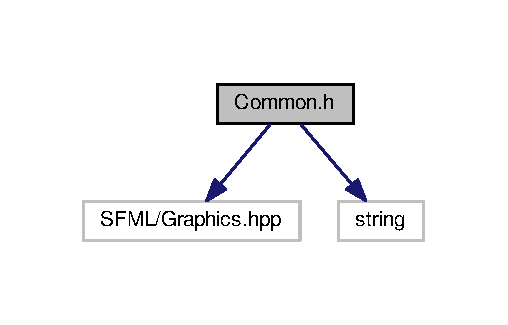
\includegraphics[width=244pt]{Common_8h__incl}
\end{center}
\end{figure}
\subsection*{Functions}
\begin{DoxyCompactItemize}
\item 
double \hyperlink{Common_8h_ae7ecf382f2e8c76a0196587e899a7c2c}{length} (const double \&x, const double \&y)\hypertarget{Common_8h_ae7ecf382f2e8c76a0196587e899a7c2c}{}\label{Common_8h_ae7ecf382f2e8c76a0196587e899a7c2c}

\begin{DoxyCompactList}\small\item\em Returns length of a vector (x, y) \end{DoxyCompactList}\item 
double \hyperlink{Common_8h_ad66815a0abad039f09fd6a2356e89045}{length\+Square} (const double \&x, const double \&y)\hypertarget{Common_8h_ad66815a0abad039f09fd6a2356e89045}{}\label{Common_8h_ad66815a0abad039f09fd6a2356e89045}

\begin{DoxyCompactList}\small\item\em Returns length$^\wedge$2 of a vector (x, y) \end{DoxyCompactList}\item 
double \hyperlink{Common_8h_a41027316c74f9e99c54ad60b110eb184}{dist} (const double \&x1, const double \&y1, const double \&x2, const double \&y2)\hypertarget{Common_8h_a41027316c74f9e99c54ad60b110eb184}{}\label{Common_8h_a41027316c74f9e99c54ad60b110eb184}

\begin{DoxyCompactList}\small\item\em Returns euclidean distance between vectors (x1, y1) and (x2, y2) \end{DoxyCompactList}\item 
double \hyperlink{Common_8h_a5d7508813f259ddb647ac23ed45d8dcf}{dist\+Square} (const double \&x1, const double \&y1, const double \&x2, const double \&y2)\hypertarget{Common_8h_a5d7508813f259ddb647ac23ed45d8dcf}{}\label{Common_8h_a5d7508813f259ddb647ac23ed45d8dcf}

\begin{DoxyCompactList}\small\item\em Returns square of euclidean distance between vectors (x1, y1) and (x2, y2) \end{DoxyCompactList}\item 
sf\+::\+Circle\+Shape \hyperlink{Common_8h_a3b0ff70843c24a762a5e9ce27a1cde4a}{make\+Circle} (float radius, float x, float y, sf\+::\+Color fill\+Color)
\begin{DoxyCompactList}\small\item\em A factory function for creating circles. \end{DoxyCompactList}\item 
sf\+::\+Rectangle\+Shape \hyperlink{Common_8h_af09a4aaccf0c9edf4c7fa105c31f5881}{make\+Rectangle} (float width, float height, float x, float y, sf\+::\+Color fill\+Color)
\begin{DoxyCompactList}\small\item\em A factory function for creating rectangles. \end{DoxyCompactList}\item 
sf\+::\+Rectangle\+Shape \hyperlink{Common_8h_ad7a729d93b3c6f41d7c5980569a56245}{make\+Line} (float x1, float y1, float x2, float y2, float thickness, sf\+::\+Color fill\+Color)
\begin{DoxyCompactList}\small\item\em A factory function for creating lines. \end{DoxyCompactList}\item 
sf\+::\+Text \hyperlink{Common_8h_a9ce5dca4edd098cdee910b3fbee82d63}{make\+Text} (string caption, int font\+Size, float x, float y, sf\+::\+Color color)
\begin{DoxyCompactList}\small\item\em A factory function for creating texts. \end{DoxyCompactList}\end{DoxyCompactItemize}
\subsection*{Variables}
\begin{DoxyCompactItemize}
\item 
sf\+::\+Font \hyperlink{Common_8h_a490e95f6a947282162bbe2896212a44e}{common\+Font}\hypertarget{Common_8h_a490e95f6a947282162bbe2896212a44e}{}\label{Common_8h_a490e95f6a947282162bbe2896212a44e}

\begin{DoxyCompactList}\small\item\em You should use only this font in your program. It loads font from F\+O\+N\+T\+\_\+\+P\+A\+TH defined in \hyperlink{Config_8h_source}{Config.\+h}. \end{DoxyCompactList}\end{DoxyCompactItemize}


\subsection{Detailed Description}
Contains some useful functions and common\+Font. 



\subsection{Function Documentation}
\index{Common.\+h@{Common.\+h}!make\+Circle@{make\+Circle}}
\index{make\+Circle@{make\+Circle}!Common.\+h@{Common.\+h}}
\subsubsection[{\texorpdfstring{make\+Circle(float radius, float x, float y, sf\+::\+Color fill\+Color)}{makeCircle(float radius, float x, float y, sf::Color fillColor)}}]{\setlength{\rightskip}{0pt plus 5cm}sf\+::\+Circle\+Shape make\+Circle (
\begin{DoxyParamCaption}
\item[{float}]{radius, }
\item[{float}]{x, }
\item[{float}]{y, }
\item[{sf\+::\+Color}]{fill\+Color}
\end{DoxyParamCaption}
)}\hypertarget{Common_8h_a3b0ff70843c24a762a5e9ce27a1cde4a}{}\label{Common_8h_a3b0ff70843c24a762a5e9ce27a1cde4a}


A factory function for creating circles. 


\begin{DoxyParams}{Parameters}
{\em radius} & the radius of the circle \\
\hline
{\em x} & the x-\/coordinate of the circle\textquotesingle{}s center \\
\hline
{\em y} & the y-\/coordinate of the circle\textquotesingle{}s center \\
\hline
{\em fill\+Color} & the color of the circle \\
\hline
\end{DoxyParams}
\begin{DoxyReturn}{Returns}
an sf\+::\+Circle\+Shape with center at (x, y) 
\end{DoxyReturn}
\index{Common.\+h@{Common.\+h}!make\+Line@{make\+Line}}
\index{make\+Line@{make\+Line}!Common.\+h@{Common.\+h}}
\subsubsection[{\texorpdfstring{make\+Line(float x1, float y1, float x2, float y2, float thickness, sf\+::\+Color fill\+Color)}{makeLine(float x1, float y1, float x2, float y2, float thickness, sf::Color fillColor)}}]{\setlength{\rightskip}{0pt plus 5cm}sf\+::\+Rectangle\+Shape make\+Line (
\begin{DoxyParamCaption}
\item[{float}]{x1, }
\item[{float}]{y1, }
\item[{float}]{x2, }
\item[{float}]{y2, }
\item[{float}]{thickness, }
\item[{sf\+::\+Color}]{fill\+Color}
\end{DoxyParamCaption}
)}\hypertarget{Common_8h_ad7a729d93b3c6f41d7c5980569a56245}{}\label{Common_8h_ad7a729d93b3c6f41d7c5980569a56245}


A factory function for creating lines. 


\begin{DoxyParams}{Parameters}
{\em x1} & the x-\/coordinate of first end of line \\
\hline
{\em y1} & the y-\/coordinate of first end of line \\
\hline
{\em x2} & the x-\/coordinate of second end of line \\
\hline
{\em y2} & the y-\/coordinate of second end of line \\
\hline
{\em thickness} & the thickness of the line \\
\hline
{\em fill\+Color} & the color of the line \\
\hline
\end{DoxyParams}
\begin{DoxyReturn}{Returns}
an sf\+::\+Rectangle\+Shape which is a line segment with specified thickness between (x1, y1) and (x2, y2) 
\end{DoxyReturn}
\index{Common.\+h@{Common.\+h}!make\+Rectangle@{make\+Rectangle}}
\index{make\+Rectangle@{make\+Rectangle}!Common.\+h@{Common.\+h}}
\subsubsection[{\texorpdfstring{make\+Rectangle(float width, float height, float x, float y, sf\+::\+Color fill\+Color)}{makeRectangle(float width, float height, float x, float y, sf::Color fillColor)}}]{\setlength{\rightskip}{0pt plus 5cm}sf\+::\+Rectangle\+Shape make\+Rectangle (
\begin{DoxyParamCaption}
\item[{float}]{width, }
\item[{float}]{height, }
\item[{float}]{x, }
\item[{float}]{y, }
\item[{sf\+::\+Color}]{fill\+Color}
\end{DoxyParamCaption}
)}\hypertarget{Common_8h_af09a4aaccf0c9edf4c7fa105c31f5881}{}\label{Common_8h_af09a4aaccf0c9edf4c7fa105c31f5881}


A factory function for creating rectangles. 


\begin{DoxyParams}{Parameters}
{\em width} & the width of the rect \\
\hline
{\em height} & the height of the rect \\
\hline
{\em x} & the x-\/coordinate of the rect\textquotesingle{}s center \\
\hline
{\em y} & the y-\/coordinate of the rect\textquotesingle{}s center \\
\hline
{\em fill\+Color} & the color of the rect \\
\hline
\end{DoxyParams}
\begin{DoxyReturn}{Returns}
an sf\+::\+Rectangle\+Shape with center at (x, y) 
\end{DoxyReturn}
\index{Common.\+h@{Common.\+h}!make\+Text@{make\+Text}}
\index{make\+Text@{make\+Text}!Common.\+h@{Common.\+h}}
\subsubsection[{\texorpdfstring{make\+Text(string caption, int font\+Size, float x, float y, sf\+::\+Color color)}{makeText(string caption, int fontSize, float x, float y, sf::Color color)}}]{\setlength{\rightskip}{0pt plus 5cm}sf\+::\+Text make\+Text (
\begin{DoxyParamCaption}
\item[{string}]{caption, }
\item[{int}]{font\+Size, }
\item[{float}]{x, }
\item[{float}]{y, }
\item[{sf\+::\+Color}]{color}
\end{DoxyParamCaption}
)}\hypertarget{Common_8h_a9ce5dca4edd098cdee910b3fbee82d63}{}\label{Common_8h_a9ce5dca4edd098cdee910b3fbee82d63}


A factory function for creating texts. 


\begin{DoxyParams}{Parameters}
{\em caption} & the text to be displayed \\
\hline
{\em font\+Size} & the size of characters \\
\hline
{\em x} & the x-\/coordinate of the center of text \\
\hline
{\em y} & the y-\/coordinate of the center of text \\
\hline
{\em color} & the color of text \\
\hline
\end{DoxyParams}
\begin{DoxyReturn}{Returns}
an sf\+::\+Text with center at (x, y) 
\end{DoxyReturn}

\hypertarget{Game_8h}{}\section{Game.\+h File Reference}
\label{Game_8h}\index{Game.\+h@{Game.\+h}}


Contains the main \hyperlink{classGame}{Game} class.  


{\ttfamily \#include $<$S\+F\+M\+L/\+Graphics.\+hpp$>$}\\*
{\ttfamily \#include \char`\"{}Info.\+h\char`\"{}}\\*
{\ttfamily \#include \char`\"{}Config.\+h\char`\"{}}\\*
{\ttfamily \#include \char`\"{}Game\+State.\+h\char`\"{}}\\*
{\ttfamily \#include $<$thread$>$}\\*
{\ttfamily \#include $<$mutex$>$}\\*
{\ttfamily \#include $<$sstream$>$}\\*
Include dependency graph for Game.\+h\+:\nopagebreak
\begin{figure}[H]
\begin{center}
\leavevmode
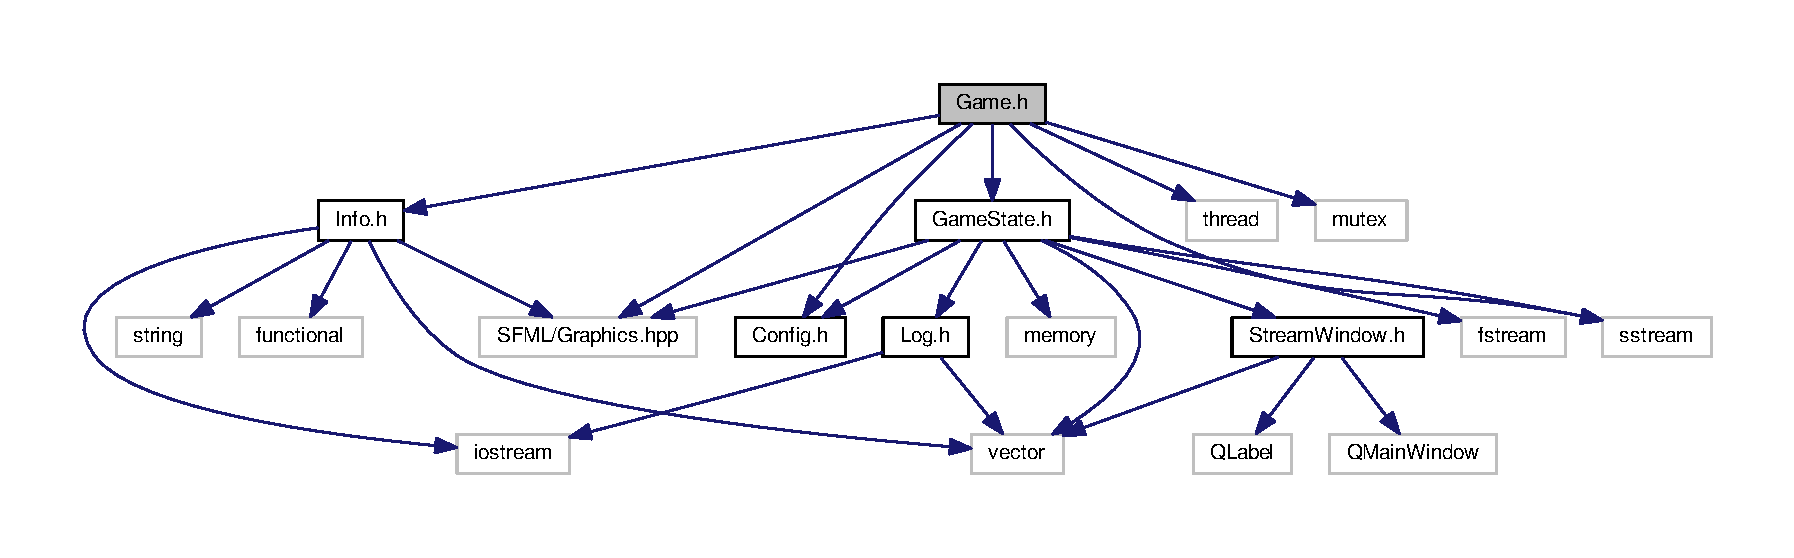
\includegraphics[width=350pt]{Game_8h__incl}
\end{center}
\end{figure}
\subsection*{Classes}
\begin{DoxyCompactItemize}
\item 
class \hyperlink{classGame}{Game}
\begin{DoxyCompactList}\small\item\em The main \hyperlink{classGame}{Game} class. You should make a derived class from it. \end{DoxyCompactList}\end{DoxyCompactItemize}


\subsection{Detailed Description}
Contains the main \hyperlink{classGame}{Game} class. 


\hypertarget{GameState_8h}{}\section{Game\+State.\+h File Reference}
\label{GameState_8h}\index{Game\+State.\+h@{Game\+State.\+h}}


Contains the \hyperlink{classGameState}{Game\+State} class.  


{\ttfamily \#include \char`\"{}Stream\+Window.\+h\char`\"{}}\\*
{\ttfamily \#include \char`\"{}Log.\+h\char`\"{}}\\*
{\ttfamily \#include \char`\"{}Config.\+h\char`\"{}}\\*
{\ttfamily \#include $<$sstream$>$}\\*
{\ttfamily \#include $<$fstream$>$}\\*
{\ttfamily \#include $<$vector$>$}\\*
{\ttfamily \#include $<$S\+F\+M\+L/\+Graphics.\+hpp$>$}\\*
{\ttfamily \#include $<$memory$>$}\\*
Include dependency graph for Game\+State.\+h\+:\nopagebreak
\begin{figure}[H]
\begin{center}
\leavevmode
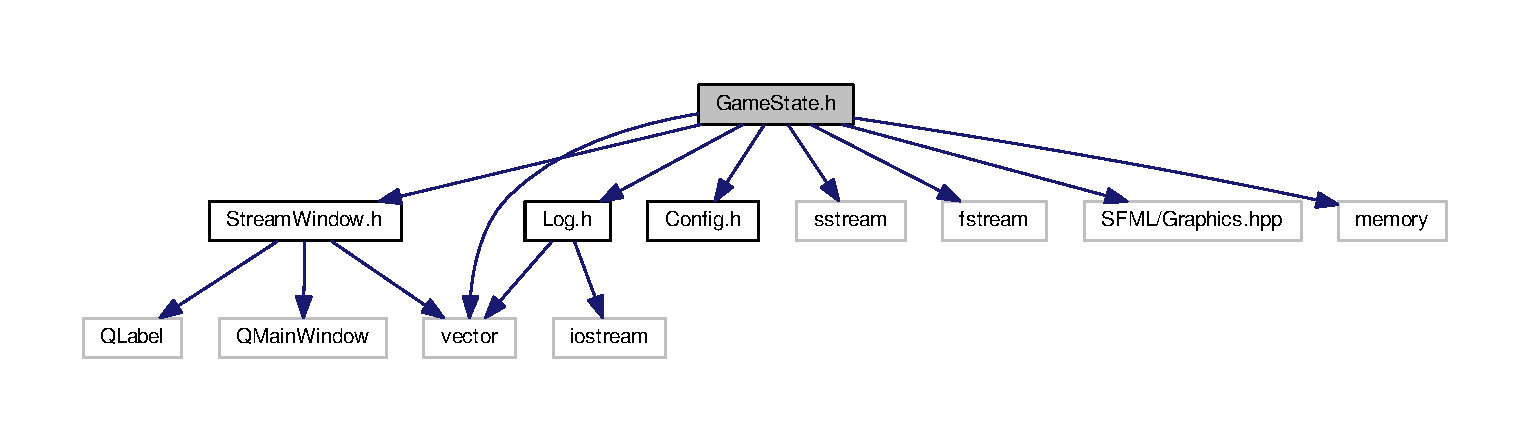
\includegraphics[width=350pt]{GameState_8h__incl}
\end{center}
\end{figure}
This graph shows which files directly or indirectly include this file\+:\nopagebreak
\begin{figure}[H]
\begin{center}
\leavevmode
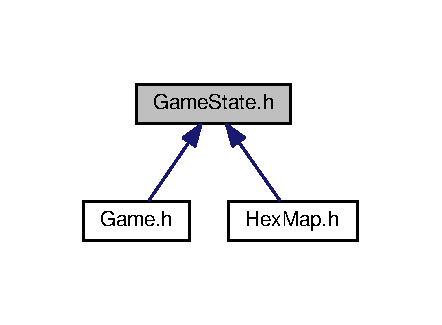
\includegraphics[width=212pt]{GameState_8h__dep__incl}
\end{center}
\end{figure}
\subsection*{Classes}
\begin{DoxyCompactItemize}
\item 
class \hyperlink{classGameState}{Game\+State}
\begin{DoxyCompactList}\small\item\em This class contains the state of the game. It draws it, shows the output window and saves game for further viewing. \end{DoxyCompactList}\end{DoxyCompactItemize}


\subsection{Detailed Description}
Contains the \hyperlink{classGameState}{Game\+State} class. 


\hypertarget{HexMap_8h}{}\section{Hex\+Map.\+h File Reference}
\label{HexMap_8h}\index{Hex\+Map.\+h@{Hex\+Map.\+h}}


Contains the \hyperlink{classHexMap}{Hex\+Map} class.  


{\ttfamily \#include $<$vector$>$}\\*
{\ttfamily \#include $<$S\+F\+M\+L/\+Graphics.\+hpp$>$}\\*
{\ttfamily \#include \char`\"{}Game\+State.\+h\char`\"{}}\\*
Include dependency graph for Hex\+Map.\+h\+:\nopagebreak
\begin{figure}[H]
\begin{center}
\leavevmode
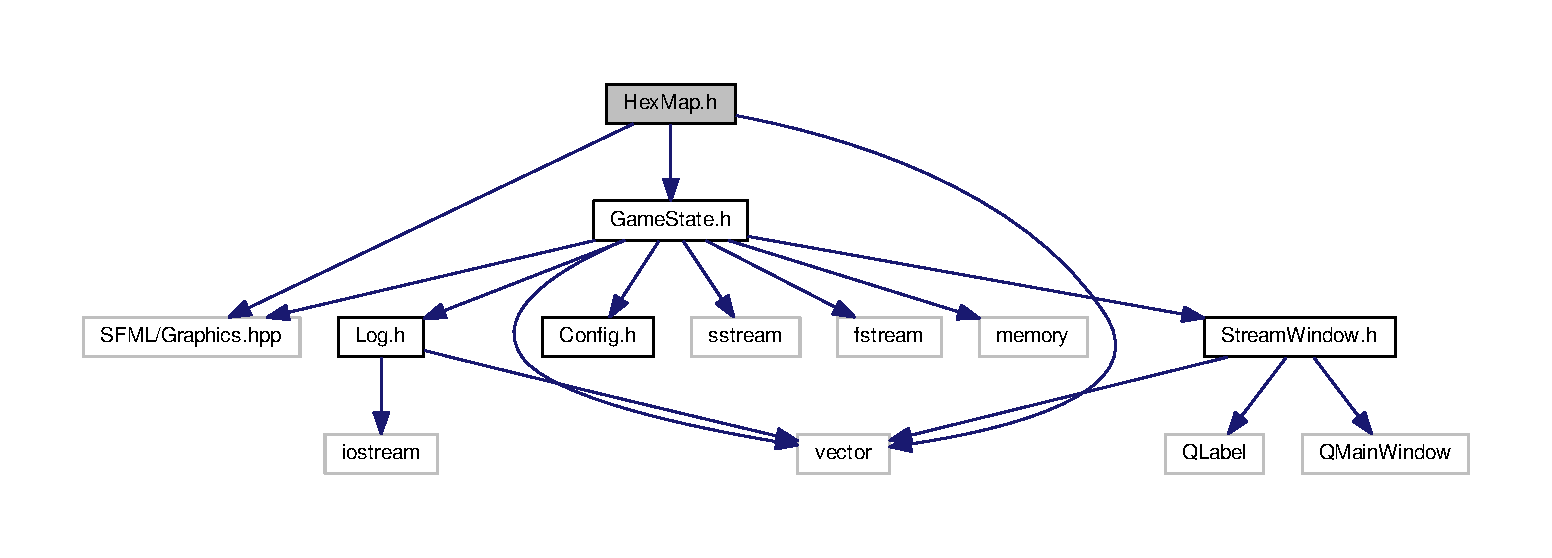
\includegraphics[width=350pt]{HexMap_8h__incl}
\end{center}
\end{figure}
\subsection*{Classes}
\begin{DoxyCompactItemize}
\item 
class \hyperlink{classHexMap}{Hex\+Map}
\begin{DoxyCompactList}\small\item\em Useful class for using hex maps. \end{DoxyCompactList}\end{DoxyCompactItemize}


\subsection{Detailed Description}
Contains the \hyperlink{classHexMap}{Hex\+Map} class. 


\hypertarget{Info_8h}{}\section{Info.\+h File Reference}
\label{Info_8h}\index{Info.\+h@{Info.\+h}}


Contains the \hyperlink{classInfo}{Info} class.  


{\ttfamily \#include $<$S\+F\+M\+L/\+Graphics.\+hpp$>$}\\*
{\ttfamily \#include $<$functional$>$}\\*
{\ttfamily \#include $<$vector$>$}\\*
{\ttfamily \#include $<$string$>$}\\*
{\ttfamily \#include $<$iostream$>$}\\*
Include dependency graph for Info.\+h\+:\nopagebreak
\begin{figure}[H]
\begin{center}
\leavevmode
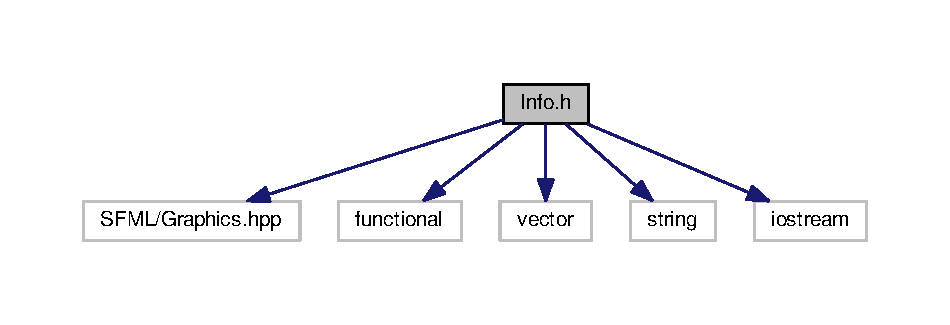
\includegraphics[width=350pt]{Info_8h__incl}
\end{center}
\end{figure}
This graph shows which files directly or indirectly include this file\+:\nopagebreak
\begin{figure}[H]
\begin{center}
\leavevmode
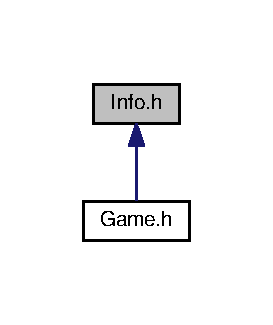
\includegraphics[width=131pt]{Info_8h__dep__incl}
\end{center}
\end{figure}
\subsection*{Classes}
\begin{DoxyCompactItemize}
\item 
class \hyperlink{classInfo}{Info}
\begin{DoxyCompactList}\small\item\em Usable class for printing real-\/time info. \end{DoxyCompactList}\end{DoxyCompactItemize}


\subsection{Detailed Description}
Contains the \hyperlink{classInfo}{Info} class. 


\hypertarget{Log_8h}{}\section{Log.\+h File Reference}
\label{Log_8h}\index{Log.\+h@{Log.\+h}}


Contains the \hyperlink{classMultiStream}{Multi\+Stream} class.  


{\ttfamily \#include $<$vector$>$}\\*
{\ttfamily \#include $<$iostream$>$}\\*
Include dependency graph for Log.\+h\+:\nopagebreak
\begin{figure}[H]
\begin{center}
\leavevmode
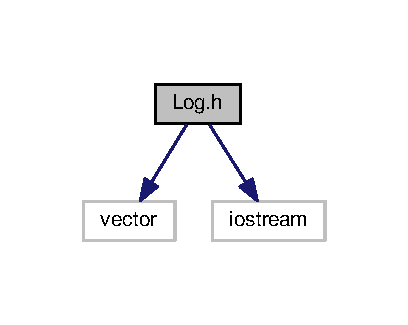
\includegraphics[width=196pt]{Log_8h__incl}
\end{center}
\end{figure}
This graph shows which files directly or indirectly include this file\+:\nopagebreak
\begin{figure}[H]
\begin{center}
\leavevmode
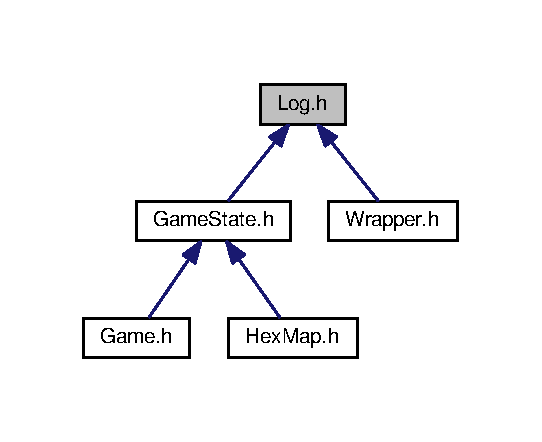
\includegraphics[width=260pt]{Log_8h__dep__incl}
\end{center}
\end{figure}
\subsection*{Classes}
\begin{DoxyCompactItemize}
\item 
class \hyperlink{classMultiStream}{Multi\+Stream}
\begin{DoxyCompactList}\small\item\em Class used to combining multiple streams into one. \end{DoxyCompactList}\end{DoxyCompactItemize}
\subsection*{Functions}
\begin{DoxyCompactItemize}
\item 
void \hyperlink{Log_8h_aeea2c66c479cd8b6361b08371bed6966}{open\+\_\+log} (ofstream \&of, string dir)
\begin{DoxyCompactList}\small\item\em Reopens the stream into a new file in a specified directory. If the directory doesn\textquotesingle{}t exist it is created. The name of the file is H\+H\+\_\+\+M\+M\+\_\+\+S\+S.\+log where HH, MM, SS is current hour, minute and second. \end{DoxyCompactList}\end{DoxyCompactItemize}
\subsection*{Variables}
\begin{DoxyCompactItemize}
\item 
\hyperlink{classMultiStream}{Multi\+Stream} \hyperlink{Log_8h_abcf4b357cfc0eadec527ad23142842d6}{mout}\hypertarget{Log_8h_abcf4b357cfc0eadec527ad23142842d6}{}\label{Log_8h_abcf4b357cfc0eadec527ad23142842d6}

\begin{DoxyCompactList}\small\item\em \hyperlink{classMultiStream}{Multi\+Stream} which initially contains only cout. \end{DoxyCompactList}\item 
\hyperlink{classMultiStream}{Multi\+Stream} \hyperlink{Log_8h_aeda56f358e2b30e8d8318ca0db6e3277}{merr}\hypertarget{Log_8h_aeda56f358e2b30e8d8318ca0db6e3277}{}\label{Log_8h_aeda56f358e2b30e8d8318ca0db6e3277}

\begin{DoxyCompactList}\small\item\em \hyperlink{classMultiStream}{Multi\+Stream} which initially contains only cerr. \end{DoxyCompactList}\end{DoxyCompactItemize}


\subsection{Detailed Description}
Contains the \hyperlink{classMultiStream}{Multi\+Stream} class. 



\subsection{Function Documentation}
\index{Log.\+h@{Log.\+h}!open\+\_\+log@{open\+\_\+log}}
\index{open\+\_\+log@{open\+\_\+log}!Log.\+h@{Log.\+h}}
\subsubsection[{\texorpdfstring{open\+\_\+log(ofstream \&of, string dir)}{open_log(ofstream &of, string dir)}}]{\setlength{\rightskip}{0pt plus 5cm}void open\+\_\+log (
\begin{DoxyParamCaption}
\item[{ofstream \&}]{of, }
\item[{string}]{dir}
\end{DoxyParamCaption}
)}\hypertarget{Log_8h_aeea2c66c479cd8b6361b08371bed6966}{}\label{Log_8h_aeea2c66c479cd8b6361b08371bed6966}


Reopens the stream into a new file in a specified directory. If the directory doesn\textquotesingle{}t exist it is created. The name of the file is H\+H\+\_\+\+M\+M\+\_\+\+S\+S.\+log where HH, MM, SS is current hour, minute and second. 


\begin{DoxyParams}{Parameters}
{\em of} & the stream to reopen \\
\hline
{\em dir} & the name of the directory \\
\hline
\end{DoxyParams}

\hypertarget{Wrapper_8h}{}\section{Wrapper.\+h File Reference}
\label{Wrapper_8h}\index{Wrapper.\+h@{Wrapper.\+h}}


Contains a few useful functions for communication with server.  


{\ttfamily \#include \char`\"{}C\+Tcp\+Fwd.\+h\char`\"{}}\\*
{\ttfamily \#include \char`\"{}Log.\+h\char`\"{}}\\*
{\ttfamily \#include $<$string$>$}\\*
{\ttfamily \#include $<$vector$>$}\\*
Include dependency graph for Wrapper.\+h\+:\nopagebreak
\begin{figure}[H]
\begin{center}
\leavevmode
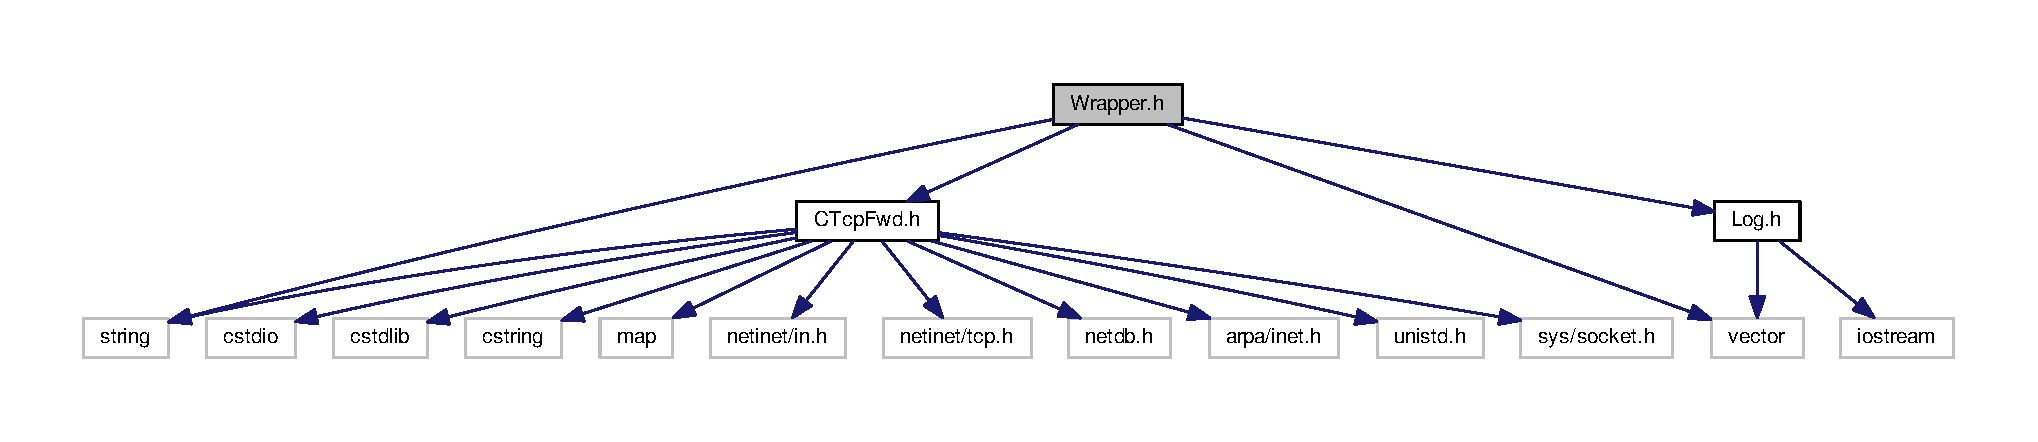
\includegraphics[width=350pt]{Wrapper_8h__incl}
\end{center}
\end{figure}
\subsection*{Functions}
\begin{DoxyCompactItemize}
\item 
void \hyperlink{Wrapper_8h_a97c4ae32c616eca02a42815ec76ecad6}{connect} (string host, int port, string login, string password)
\begin{DoxyCompactList}\small\item\em Initializes T\+CP connection. After calling this function, stdout sends output to the server and stdin reads input from it. \end{DoxyCompactList}\item 
bool \hyperlink{Wrapper_8h_a28b4da67afbeadc64a92aa05d4c05f00}{send\+Message} (string message=string())
\begin{DoxyCompactList}\small\item\em Writes message followed by endline to the stdout, and then checks if the response is OK or handles errors. \end{DoxyCompactList}\item 
void \hyperlink{Wrapper_8h_aa3b21853f890838c88d047d6c2786917}{wait} ()\hypertarget{Wrapper_8h_aa3b21853f890838c88d047d6c2786917}{}\label{Wrapper_8h_aa3b21853f890838c88d047d6c2786917}

\begin{DoxyCompactList}\small\item\em Sends W\+A\+IT message and reads 2 O\+Ks. \end{DoxyCompactList}\item 
int \hyperlink{Wrapper_8h_a6b883c8cf0bdd74badc0fd04c7e94ca9}{turns\+Left} ()
\begin{DoxyCompactList}\small\item\em Calls T\+U\+R\+N\+S\+\_\+\+L\+E\+F\+T\+\_\+\+C\+O\+M\+M\+A\+ND (defined in \hyperlink{Config_8h_source}{Config.\+h}) and reads the response. \end{DoxyCompactList}\end{DoxyCompactItemize}


\subsection{Detailed Description}
Contains a few useful functions for communication with server. 



\subsection{Function Documentation}
\index{Wrapper.\+h@{Wrapper.\+h}!connect@{connect}}
\index{connect@{connect}!Wrapper.\+h@{Wrapper.\+h}}
\subsubsection[{\texorpdfstring{connect(string host, int port, string login, string password)}{connect(string host, int port, string login, string password)}}]{\setlength{\rightskip}{0pt plus 5cm}void connect (
\begin{DoxyParamCaption}
\item[{string}]{host, }
\item[{int}]{port, }
\item[{string}]{login, }
\item[{string}]{password}
\end{DoxyParamCaption}
)}\hypertarget{Wrapper_8h_a97c4ae32c616eca02a42815ec76ecad6}{}\label{Wrapper_8h_a97c4ae32c616eca02a42815ec76ecad6}


Initializes T\+CP connection. After calling this function, stdout sends output to the server and stdin reads input from it. 


\begin{DoxyParams}{Parameters}
{\em host} & the name of the host \\
\hline
{\em port} & the port number (integer) \\
\hline
{\em login} & team login \\
\hline
{\em password} & team password \\
\hline
\end{DoxyParams}
\index{Wrapper.\+h@{Wrapper.\+h}!send\+Message@{send\+Message}}
\index{send\+Message@{send\+Message}!Wrapper.\+h@{Wrapper.\+h}}
\subsubsection[{\texorpdfstring{send\+Message(string message=string())}{sendMessage(string message=string())}}]{\setlength{\rightskip}{0pt plus 5cm}bool send\+Message (
\begin{DoxyParamCaption}
\item[{string}]{message = {\ttfamily string()}}
\end{DoxyParamCaption}
)}\hypertarget{Wrapper_8h_a28b4da67afbeadc64a92aa05d4c05f00}{}\label{Wrapper_8h_a28b4da67afbeadc64a92aa05d4c05f00}


Writes message followed by endline to the stdout, and then checks if the response is OK or handles errors. 


\begin{DoxyParams}{Parameters}
{\em message} & the message to write \\
\hline
\end{DoxyParams}
\begin{DoxyReturn}{Returns}
true if server returned OK, false otherwise 
\end{DoxyReturn}
\index{Wrapper.\+h@{Wrapper.\+h}!turns\+Left@{turns\+Left}}
\index{turns\+Left@{turns\+Left}!Wrapper.\+h@{Wrapper.\+h}}
\subsubsection[{\texorpdfstring{turns\+Left()}{turnsLeft()}}]{\setlength{\rightskip}{0pt plus 5cm}int turns\+Left (
\begin{DoxyParamCaption}
{}
\end{DoxyParamCaption}
)}\hypertarget{Wrapper_8h_a6b883c8cf0bdd74badc0fd04c7e94ca9}{}\label{Wrapper_8h_a6b883c8cf0bdd74badc0fd04c7e94ca9}


Calls T\+U\+R\+N\+S\+\_\+\+L\+E\+F\+T\+\_\+\+C\+O\+M\+M\+A\+ND (defined in \hyperlink{Config_8h_source}{Config.\+h}) and reads the response. 

\begin{DoxyReturn}{Returns}
the number of turns left 
\end{DoxyReturn}

%--- End generated contents ---

% Index
\backmatter
\newpage
\phantomsection
\clearemptydoublepage
\addcontentsline{toc}{chapter}{Index}
\printindex

\end{document}
